As the purpose of the project is to create a system in which a user should be able to see the weather forecast for a specific area, or more precisely, the temperature forecast, we have developed a system that leverages several models to perform the temperature forecasting. 
The goal is to allow the user to interact with the system in such a way that the user can see the accuracy of the different models. 
On a web page, the user is able to select a city for which they want to predict the temperature. The results are shown both as a graph that displays the predicted value versus the actual value, as well as the specific set of temperatures of that city for a given time period into the future. This is similar to what one may see on regular weather forecasts.

In order to achieve, this we have constructed a pipeline that preprocesses the data, trains our models, and the resulting models are then used to perform the forecasting displayed on a web application. 
Figure \ref{fig:architecture diagram} shows an overview of the architecture of the pipeline.

Note that since the transformer model is the best performing model, which is shown in section (experiment afsnit), this is the model that we chose to include and describe as part of the pipeline. Regardless of this fact, the other models are used in the pipeline in a similar fashion.

In section \ref{sec:data loading and preprocessing}, we start by presenting the data loading and preprocessing phase of the system architecture, and we also motivate our interest in the transformer model.
Then, in sections \ref{sec:self-attention mechanism} and \ref{sec:multi-head attention}, we describe preliminary theory about the transformer model; the self-attention mechanism and multi-head attention module. 
Afterwards, in section \ref{sec:time2vec} we introduce the method we use for embedding temporal information into the transformer model. 
In section \ref{sec:training}, we describe our approach to training the models, and how we serialize the formatted data and trained models into the Python \texttt{pickle} format.
Finally, in section \ref{sec:web app}, we introduce the front-end web application where the user is able to make predictions using our trained models using a simple graphical user interface in a web browser.



\begin{figure*}
	\centering
	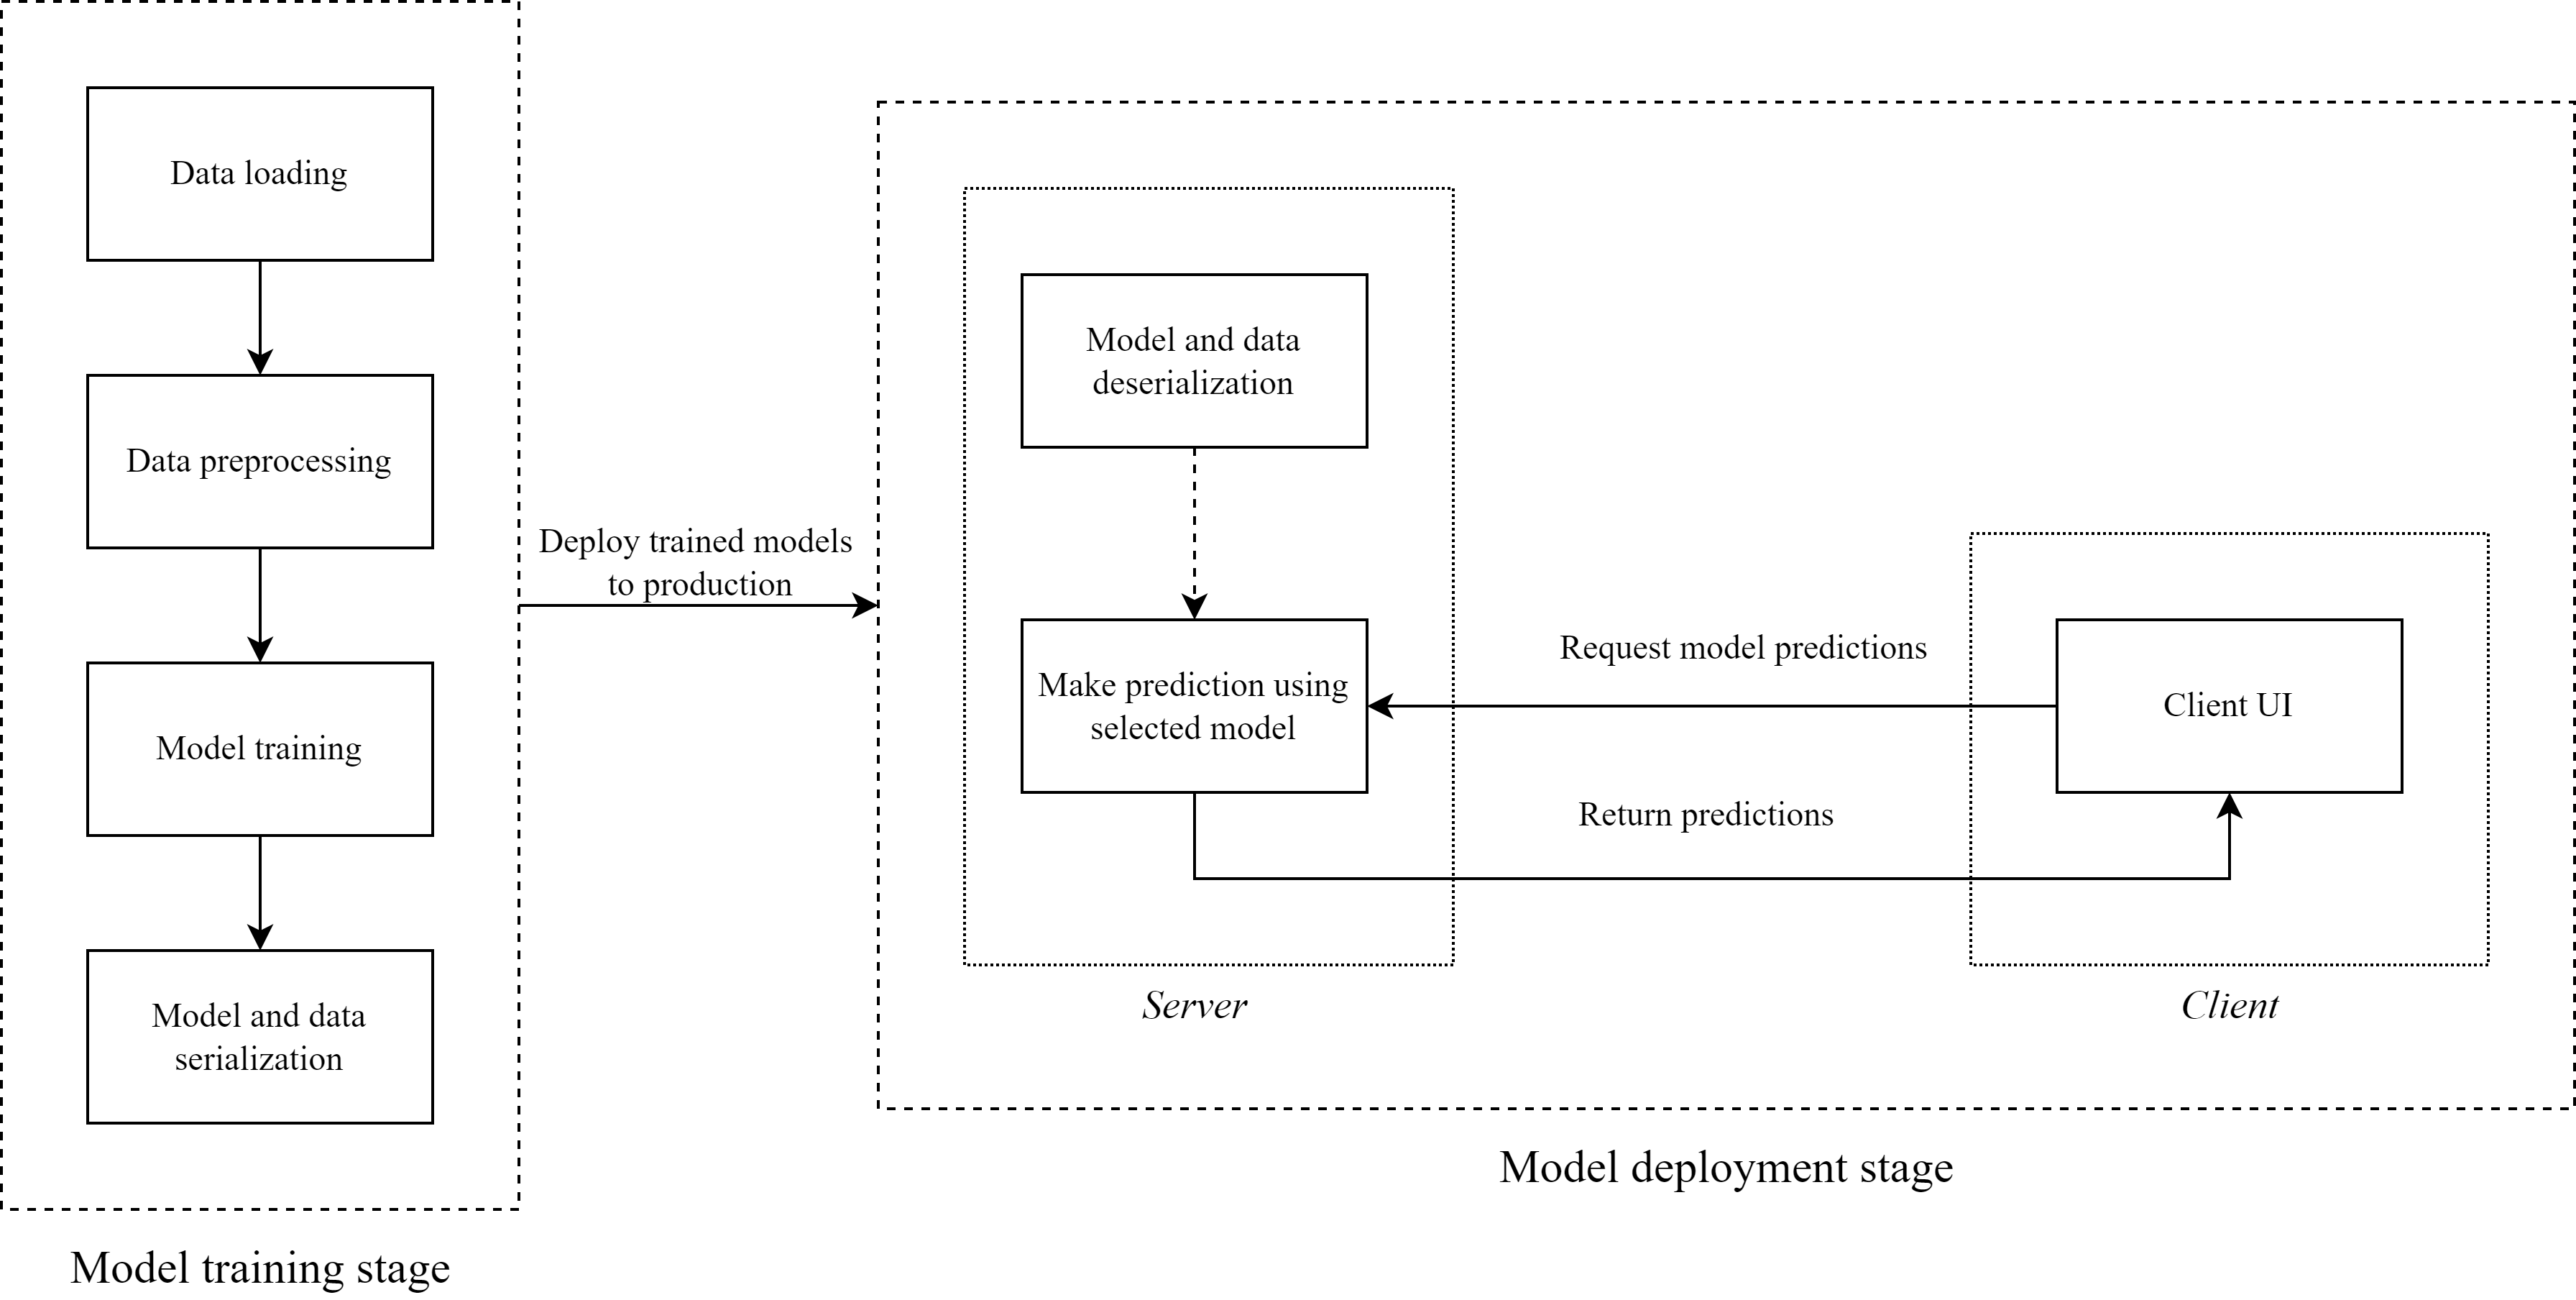
\includegraphics[width=1\textwidth]{Architecture diagram}
	\caption{The architecture of the system pipeline.}
	\label{fig:architecture diagram}
\end{figure*}